\chapter[Introdução]{Introdução}

	\section[Problema]{Problema}

	Tirar chopp é uma arte.  Não há muito que se discutir, ao se conversar com 
	apreciadores \textit{sommeliers} do mesmo, eles hão de concordar que isso 
	deve ser feito com paixão, dedicação  e técnica,  para que se obtenha o máximo de 
	qualidade. Requisitos que muitas vezes não são cumpridos por aqueles que servem o
	chopp como emprego.
	
	Dado o custo  envolvido com o trabalho de garçons, demora no atendimento,
	falta de praticidade, ausência de padronização na tiragem do chopp e problemas de
	controle de temperatura, os quais contribuem para a desvalorização do produto,
	prejudicam o seu consumo, bem como encarecem o mesmo, deseja-se 
	minimizar as ocorrências do que  foi citado. 	
	
	\section[Estado da Arte]{Estado da Arte}
	
	No mundo inteiro, a cada dia, mais e mais pessoas se deixam seduzir pelo insuperável sabor das bebidas fermentadas, como a cerveja, e particularmente o chopp. Assim sendo esse permite a existência de um mercado que estimule a criatividade de muitos empreendedores.  

	Hodiernamente a bebida é um atrativo para casas noturnas e eventos que ao longo dos anos ganhou vários apreciadores,possuindo inclusive eventos voltados apenas para os degustadores da bebida. 

	Um exemplo é o sistema myTapp de uma startup de Florianópolis.  O sistema faz a venda de chopp ao estilo 
	\textit{self-service}, no qual os usuários compram créditos para uso da máquina e podem colocar somente a quantidade que 
	consumirem. Esse sistema favorece novatos no consumo de chopp que têm a oportunidade de serem cobrados somente 
	pelo que consumirem, podendo provar diversos tipos de chopp. A figura \ref{exemplo-chopp} mostra o uso desse sistema.

	\begin{figure}[H]
		\centering
		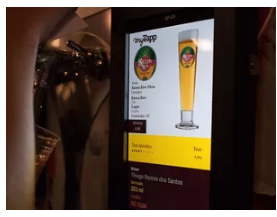
\includegraphics[scale= 0.9]{figuras/exemplo-chopp.png}
		\caption{Exemplo de chopeira automatizada.}
		\label{exemplo-chopp}
	\end{figure}

	Outro exemplo de equipamento de ponta é uma chopeira  que se encontra no Japão. Ela é capaz de servir de forma 
	automática os copos e localiza-se no Aeroporto Internacional de Kansai (KIX) em Osaka. A foto da mesma encontra-se 
	na imagem \ref{exemplo-japao}.

	\begin{figure}[!htb]
		\centering
		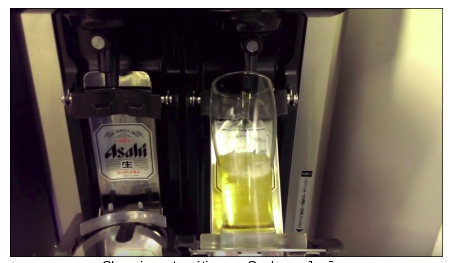
\includegraphics[scale= 0.9]{figuras/exemplo-japao.png}
		\caption{Chopeira automática de Osaka.}
		\label{exemplo-japao}
	\end{figure}

	\section[Objetivos]{Objetivos}
		\subsection[Geral]{Geral}
			Construir uma chopeira que realiza a venda e a tiragem de chopp de forma automatizada, seguindo o 
			paradigma de uma \textit{Vending Machine}. 

		\subsection[Específico]{Específico}
			\begin{itemize}
				\item Servir automaticamente o chopp.
				\item Comprovar autenticação da compra previamentp efetuada.
				\item Efetivar a compra  de forma online. 
				\item Realizar o controle e monitoramento eletrônicp de temperatura de forma automatizada.
				\item Inclinar o copo, de acordo com os padrões de tiragem de chopp.
				\item Controlar a quantidade de espuma no copo (colarinho) de acordo com a escolha do usuário e padrões predefinidos .
				\item Selecionar a quantidade de chopp a ser servida, de acordo com padrões prévios.
				\item Fornecer energia de forma suplementar em casos emergenciais.
				\item Permitir a escolha entre dois tipos de chopp
			\end{itemize}
	
	\section[Escopo]{Escopo}
		Trata-se de uma solução de venda remota para compra de chopp no cartão, servindo com preferências predefinidas 
		(colarinho, quantidade e tipo), realizando a venda de forma autônoma otimizando a tiragem do chopp. Essa 
		solução é obtida a partir de um sistema que possui alimentação redundante de energia por um certo período de 
		tempo, fazendo parte de um sistema para controle da quantidade e das vendas de chopp. O escopo não engloba a o 
		congelamento do chopp; a produção do chopp ou de seu gás; a venda de drinks, cerveja, refrigerantes e 
		alimentos; o pagamento via dinheiro em espécie; uma máquina outdoor; a troca automática do chopp (feito 
		manualmente) e o reuso do copo, assumindo que os copos que serão consumidos serão reusados.

	\section[Termo de Abertura do Projeto]{Termo de Abertura do Projeto}
		O Termo de Abertura de Projeto objetiva formalizar o início do projeto AutoChopp, onde ocorrerá o planejamento 
		inicial de custos, restrições, riscos, tempo, cronograma e marcos. 

		\subsection[Descrição do Projeto]{Descrição do Projeto}
			Para ter uma visão clara do projeto, foi usado o mapeamento de atividade no modelo 5W2H, que está descrito 
			a seguir:
			\begin{enumerate}
				\item \textit{What?}
					\begin{itemize}
						\item Uma \textit{vending-machine} de chopp;
						\item Uma máquina como serviço
					\end{itemize}
				\item \textit{Why}?
					\begin{itemize}
						\item Reduzir custos com mão de obra;
						\item Praticidade para servir o chopp;
						\item Praticidade na compra e consumo;
						\item Facilidade em gerenciar o consumo;
						\item Agregar valor com Inovação e tecnologia	
					\end{itemize}
				\item \textit{Where}?
					\begin{itemize}
						\item No campus Gama da faculdade de Brasília;
						\item República Kzona;
						\item Galpão da FGA;
						\item Laboratório NEI;
						\item Laboratório de Materiais
					\end{itemize}
				\item \textit{When}?
					\begin{itemize}
						\item No período do segundo semestre de 2017
					\end{itemize}
				\item \textit{Who}?
					\begin{itemize}
						\item Alunos dos Cursos de Engenharias da Universidade de Brasília Campus Gama que cursam a 	disciplina Projeto Integrador 2
					\end{itemize}
			\end{enumerate}

			\begin{enumerate}
				\item \textit{How}?
					\begin{itemize}
						\item Utilizando os conhecimentos dos membros do projeto e orientação dos professores da disciplina Projeto Integrador 2.
					\end{itemize}
				\item \textit{How Much}?
					\begin{itemize}
						\item O custo do projeto pode ser conferido na tabela \ref{custos}
					\end{itemize}
			\end{enumerate}

		\subsection[Propósito e justificativa do Projeto]{Propósito e justificativa do Projeto}
			O Projeto tem como objetivo oferecer a donos de bares e restaurantes uma maneira prática de servir chopp a seus clientes. Assim, o cliente pode ter mais autonomia para escolher as preferências em relação ao seu chopp e retirá-lo na máquina. Com todo esse processo de automatização, os donos desses estabelecimentos podem reduzir custos com garçons, demora no atendimento, falta de praticidade, e aumentar a qualidade do chopp servido.
		
		\subsection[Restrições do Projeto]{Restrições do Projeto}
			Legislação
			\textit{De acordo com a legislação brasileira, especificamente o ECA (Estatuto da Criança e do Adolescente), é crime contra a criança e o adolescente, por ação ou omissão, sem prejuízo do disposto na legislação penal: “vender, fornecer, servir, ministrar ou entregar, ainda que gratuitamente, de qualquer forma, a criança ou a adolescente, bebida alcoólica ou, sem justa causa, outros produtos cujos componentes possam causar dependência física ou psíquica”. Tal crime tem pena de detenção de 2 (dois) a 4 (quatro) anos, e multa, se o fato não constitui crime mais grave. Além disso, a lei ainda se refere expressamente a proibição da venda de bebidas alcoólicas à criança ou ao adolescente, estabelecendo pena: de multa de R\$\ 3.000,00 (três mil reais) a R\$\ 10.000,00 (dez mil reais) e de medida administrativa de interdição do estabelecimento comercial até o recolhimento da multa aplicada. Dessa forma, toda a construção do projeto deve levar em conta que não será possível vender chopp aos menores de idade.
			}

		\subsection[Riscos do Projeto]{Riscos do Projeto}
			
			\subsubsection[Riscos de Estrutura]{Riscos de Estrutura}
				% Please add the following required packages to your document preamble:
				% \usepackage{graphicx}
				\begin{table}[H]
				\centering
				\caption{Riscos do Projeto de Estrutura}
				\label{riscos-estrutura}
				\resizebox{\textwidth}{!}{%
				\begin{tabular}{|c|c|c|c|c|}
				\hline
				\textbf{Risco} & \textbf{Consequência} & \textbf{Probabilidade} & \textbf{Impacto} & \textbf{Ação Estratégica} \\ \hline
				\begin{tabular}[c]{@{}c@{}}Design preliminar não atende aos \\ requisitos do projeto\end{tabular} & \begin{tabular}[c]{@{}c@{}}Não aceitação do design \\ preliminar pelos clientes.\end{tabular} & Média & Alto & \begin{tabular}[c]{@{}c@{}}Elaboração de um design que atenda\\  aos requisitos, considerando pesquisa\\ de possíveis usuários.\end{tabular} \\ \hline
				\begin{tabular}[c]{@{}c@{}}Estrutura não suportar \\ as solicitações impostas\\  pelas cargas\end{tabular} & \begin{tabular}[c]{@{}c@{}}Surgimento de trincas\\  e possível colapso \\ estrutural\end{tabular} & Baixa & Alto & \begin{tabular}[c]{@{}c@{}}Reforço e aumento \\ da rigidez estrutural\end{tabular} \\ \hline
				\begin{tabular}[c]{@{}c@{}}Qualidade de acabamento\\  inferior ao desejável\\  pelos requisitos\\  de projeto\end{tabular} & \begin{tabular}[c]{@{}c@{}}Impacto na imagem\\  e aceitação do produto\\  pelos consumidores\end{tabular} & Baixa & Alto & \begin{tabular}[c]{@{}c@{}}Melhorar a qualidade\\  dos materiais, os \\ encaixes e montagens.\end{tabular} \\ \hline
				Capacidade construtiva & Problemas com prazo & Baixa & Muito Alto & \begin{tabular}[c]{@{}c@{}}Realocação de trabalhos \\ entre membros e \\ reorganização de gestão\end{tabular} \\ \hline
				\end{tabular}%
				}
				\end{table}

			\subsubsection[Riscos de Energia]{Riscos de Energia}

				% Please add the following required packages to your document preamble:
				% \usepackage{graphicx}
				\begin{table}[H]
				\centering
				\caption{Riscos do Projeto de Energia}
				\label{riscos-energia}
				\resizebox{\textwidth}{!}{%
				\begin{tabular}{|c|c|c|c|c|}
				\hline
				\textbf{Risco} & \textbf{Consequência} & \textbf{Probabilidade} & \textbf{Impacto} & \textbf{Ação Estratégica} \\ \hline
				\begin{tabular}[c]{@{}c@{}}Atrasos no cronograma\\  da equipe.\end{tabular} & \begin{tabular}[c]{@{}c@{}}Não cumprimento do projeto \\ no tempo esperado.\end{tabular} & Média & Muito impactante & \begin{tabular}[c]{@{}c@{}}Ter um gerenciamento de \\ projeto eficiente e planejar\\  um cronograma \\ facilmente executável.\end{tabular} \\ \hline
				\begin{tabular}[c]{@{}c@{}}Motocompressor do sistema de \\ refrigeração não funcionar\end{tabular} & Nao refrigeramento do chopp & Baixa & Muito Impactante & \begin{tabular}[c]{@{}c@{}}Dimensionar corretamente o sistema\\  de refrigeração e realizar\\  os devidos testes.\end{tabular} \\ \hline
				\end{tabular}%
				}
				\end{table}

			\subsubsection[Riscos de Eletrônica]{Riscos de Eletrônica}
				% Please add the following required packages to your document preamble:
				% \usepackage{graphicx}
				\begin{table}[H]
				\centering
				\caption{Riscos do Projeto de Eletrônica}
				\label{riscos-eletronica}
				\resizebox{\textwidth}{!}{%
				\begin{tabular}{|c|c|c|c|c|}
				\hline
				\textbf{Risco} & \textbf{Consequência} & \textbf{Probabilidade} & Impacto & Ação/Estratégica \\ \hline
				\begin{tabular}[c]{@{}c@{}}Queima de \\ componente.\end{tabular} & \begin{tabular}[c]{@{}c@{}}Perda de tempo e \\ de dinheiro.\end{tabular} & Média. & Muito Alto & \begin{tabular}[c]{@{}c@{}}Fazer medições de \\ corrente e tensão precisamente\end{tabular} \\ \hline
				\begin{tabular}[c]{@{}c@{}}Erro grande de \\ medição dos sensores\end{tabular} & \begin{tabular}[c]{@{}c@{}}Análise incorreta dos \\ fatos ocorridos na \\ máquina em funcionamento\end{tabular} & Baixa & Muito Alto & \begin{tabular}[c]{@{}c@{}}Utilizar metodologias de \\ diminuição de erros\\  a partir de redundância.\end{tabular} \\ \hline
				\begin{tabular}[c]{@{}c@{}}Sistema de alimentação \\ emergencial não \\ operar corretamente\end{tabular} & \begin{tabular}[c]{@{}c@{}}Falta de refrigeração \\ quando houver falta\\  de energia \\ da concessionária\end{tabular} & Média & Baixo & \begin{tabular}[c]{@{}c@{}}Realizar um projeto\\  que consiga suportar\\  altos valores de\\  corrente média\end{tabular} \\ \hline
				\begin{tabular}[c]{@{}c@{}}Software embarcado\\  mal desenvolvido\end{tabular} & \begin{tabular}[c]{@{}c@{}}Mau processamento das\\  informações de entrada\\  e saída do controlador\end{tabular} & Baixa & \begin{tabular}[c]{@{}c@{}}Muito \\ Alto\end{tabular} & \begin{tabular}[c]{@{}c@{}}Utilizar metodologia de \\ revisões de softwares de\\  diferentes integrantes e após\\  implementação testar \\ o sistema com casos extremos.\end{tabular} \\ \hline
				\end{tabular}%
				}
				\end{table}

			\subsubsection[Riscos de Software]{Riscos de Software}
				% Please add the following required packages to your document preamble:
				% \usepackage{graphicx}
				\begin{table}[H]
				\centering
				\caption{Riscos do Projeto de Software}
				\label{risco-software}
				\resizebox{\textwidth}{!}{%
				\begin{tabular}{|c|c|c|c|c|}
				\hline
				\textbf{Risco} & \textbf{Consequência} & \textbf{Probabilidade} & Impacto & Ação/Estratégica \\ \hline
				\begin{tabular}[c]{@{}c@{}}Não conseguir \\ integrar os subsistemas\end{tabular} & \begin{tabular}[c]{@{}c@{}}Não conseguir \\ entregar o produto\end{tabular} & Alto & Muito Alto & \begin{tabular}[c]{@{}c@{}}Cumprimento\\  do cronograma\end{tabular} \\ \hline
				\begin{tabular}[c]{@{}c@{}}Não dominar as tecnologias\\  para o desenvolvimento \\ dos subsistemas.\end{tabular} & \begin{tabular}[c]{@{}c@{}}Não conseguir \\ entregar o produto\end{tabular} & Médio & Muito Alto & \begin{tabular}[c]{@{}c@{}}Cumprimento\\  do cronograma\end{tabular} \\ \hline
				\begin{tabular}[c]{@{}c@{}}Não conseguir usar a api \\ para efetuar pagamentos\end{tabular} & \begin{tabular}[c]{@{}c@{}}Não entregar o\\  produto planejado\end{tabular} & Baixa & Alto & \begin{tabular}[c]{@{}c@{}}Estudar o\\  uso correto da api\end{tabular} \\ \hline
				\begin{tabular}[c]{@{}c@{}}Não conseguir gerar o \\ QR code para \\ leitura na máquina\end{tabular} & \begin{tabular}[c]{@{}c@{}}Não entregar o\\  produto planejado.\end{tabular} & Baixa & Médio & \begin{tabular}[c]{@{}c@{}}Estudar como gerar\\  o QRcode corretamente\end{tabular} \\ \hline
				\end{tabular}%
				}
				\end{table}


		\subsection[Custos do Projeto]{Custos do Projeto}

			O custo existente no projeto relativo aos recursos humanos refere-se ao valor gasto com toda equipe presente em seu desenvolvimento e gestão.

			O valor médio de um aluno de Engenharia da UnB, de acordo com o Relatório de Gestão 2015, é R\$\ 1.020,00. Levando em consideração o tempo de curso de 5 anos (10 semestres) e a necessidade da obtenção de 240 créditos para a graduação, estima-se que cada aluno pegue 24 créditos por semestre,e, por isso, 48 por ano. Como cada crédito é estimado em 15 horas por aula tem-se o seguinte custo por hora de cada aluno:

			\begin{equation}
				{11020 \over{15 \times 48}} \cong {R\$\ 15,30}
			\end{equation}

			Visto que o projeto tem duração de 15 semanas e cada aluno irá dedicar 10 horas semanais ao projeto, haverá um esforço de 150 horas para a disciplina durante o semestre. Sendo assim, se multiplicarmos o custo por hora do aluno que é igual a R\$\ 15,30 pelas horas trabalhadas no semestre, que são 150 horas, teremos um gasto de R\$\ 2.295,00 por aluno.

			Como a equipe é composta por 13 integrantes teremos um custo total de 13 x R\$\ 2.295,00, totalizando R\$\ 29.835,00.

		\subsection[\textit{Stakeholders}]{\textit{Stakeholders}}

			\subsubsection[Cliente]{Cliente}
				Donos de bares e restaurantes.
			
			\subsubsection[Equipe de Gerência]{Equipe de Gerência}
				Membros do projeto que tem como responsabilidade o planejamento, controle e monitoramento do projeto, garantindo assim a qualidade do produto. São eles:

				\begin{table}[H]
				\centering
				\caption{Gerentes de Projeto}
				\label{gerentes}
				\begin{tabular}{|c|c|}
				\hline
				\textbf{Aluno} & \textbf{Posição} \\ \hline
				Phelipe Wener & Gerente Geral \\ \hline
				Gabriela Volpato & Gerente de Energia \\ \hline
				Victor Henrique & Gerente de Software \\ \hline
				Felipe Côrrea & Gerente de Estrutura \\ \hline
				Oziel da Silva & Gerente de Eletrônica \\ \hline
				\end{tabular}
				\end{table}					

			\subsubsection[Equipe de Desenvolvimento]{Equipe de Desenvolvimento}
				Membros que tem a função de construir o produto e toda documentação necessária. São eles: Ithallo Junior, Lucas Raposo, Gabriel Henrique, Filipe Ribeiro, Edson Gomes, Clóves Júnior, Jéssica Brito e Guilherme Matias.

			\subsubsection[Docentes]{Docentes}

				Professores da disciplina de Projeto Integrador 2 no 2º semestre de 2017 que tem como responsabilidade avaliar o produto a ser entregue. São eles: Alex Reis, Sebastien Rondineau, Rhander Viana e Paulo Meirelles.

		\subsection[Produto do Projeto]{Produto do Projeto}
			As entregas do produto serão divididas em três pontos de controle:
			\begin{itemize}
				\item Ponto de Controle 1 : Entendimento do problema,  concepção da arquitetura básica da solução e organização gerencial do projeto.
				\item Ponto de Controle 2: Projeto e desenvolvimento de Subsistemas.
				\item Ponto de Controle 3: Integração dos subsistemas e entrega do produto.
			\end{itemize}

